\documentclass[tikz,border=2pt]{standalone}
\usepackage{amsmath}
\usepackage{pgfplots}
\pgfplotsset{compat=1.18}

\begin{document}
% Reduced cost of a variable that is zero at the optimum: forcing it up to a level t changes
% the (re-optimised) objective at the rate of its reduced cost; the coefficient must improve
% by at least that amount before the variable enters the solution.
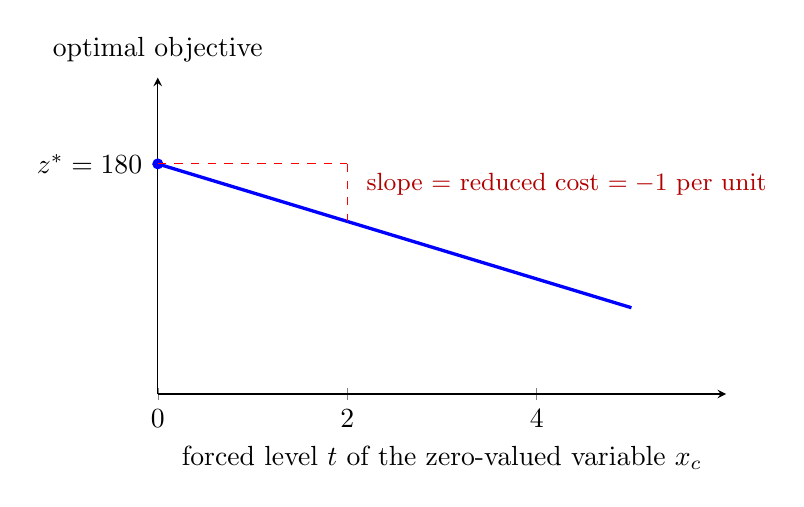
\begin{tikzpicture}
	\begin{axis}[
		axis lines=left, xmin=0, xmax=6, ymin=172, ymax=183,
		xtick={0,2,4}, ytick={180}, yticklabels={$z^\ast=180$},
		xlabel={forced level $t$ of the zero-valued variable $x_c$}, ylabel={optimal objective}, ylabel style={rotate=-90, anchor=south, at={(axis description cs:0,1.02)}},
		width=8.8cm, height=5.6cm, clip=false
		]
		\addplot[blue, very thick, domain=0:5, samples=2] {180-x};
		\fill[blue] (axis cs:0,180) circle (2pt);
		\draw[red, dashed] (axis cs:2,180) -- (axis cs:2,178);
		\draw[red, dashed] (axis cs:0,180) -- (axis cs:2,180);
		\node[red!70!black, font=\small, anchor=west] at (axis cs:2.1,179.3) {slope $=$ reduced cost $=-1$ per unit};
	\end{axis}
	\end{tikzpicture}
\end{document}
